\chapter{Análise de Complexidade do Particionamento de Blocos do AV1}
\label{cap:5}

Durante a revisão sistemática da literatura, ficou claro que o uso de particionamento de blocos para reaproveitamento de informações é uma das principais formas para acelerar a transcodificação de vídeo. Para demonstrar o impacto que as estruturas de particionamento ocasionam na codificação do vídeo, neste capítulo analisamos a complexidade do codificador AV1, principalmente em relação ao custo computacional e o impacto na eficiência de codificação relacionado ao processo de particionamento.

Anteriormente, na seção \ref{cap:3.3}, apresentamos, na Tabela \ref{tab:V}, os tamanhos de blocos e os particionamentos permitidos em alguns formatos de codificação de vídeo. A estrutura de particionamento de blocos do AV1 é representada por uma árvore de particionamentos, cujos nós intermediários possuem quatro filhos. O nó raiz, denominado Superbloco (SB), possui dois tamanhos válidos: o principal, de 128$\times$128 amostras, e o segundo, de 64$\times$64 amostras, sendo este último utilizado principalmente em vídeos de baixa resolução. Já o menor bloco permitido no AV1 também depende da resolução do vídeo, sendo que o principal tamanho é de 4$\times$4, exceto caso a resolução seja igual ou superior a UHD4K. Neste caso, o menor tamanho de bloco permitido é de 8$\times$8 amostras. Por fim, existem 21 possibilidades de nós folhas no AV1, como mostramos na Tabela \ref{tab:V}, variando entre blocos quadráticos e blocos retangulares de proporção 1:2, 2:1, 4:1 e 1:4. É importante observar que as predições intraquadro ou interquadros são permitidas apenas nos nós folhas. Logo, durante a codificação são avaliadas diferentes configurações de árvores, cada uma com diferentes conjuntos de nós folhas.

Como qualquer estrutura de dados do tipo árvore, a árvore de particionamentos do AV1 possui profundidades bem definidas, mais especificamente seis, que podem ser facilmente associadas ao tamanho de bloco quadrático principal daquela profundidade, sendo: 0 para 128$\times$128, 1 para 64$\times$64, 2 para 32$\times$32, 3 para 16$\times$16, 4 para 8$\times$8 e 5 para 4$\times$4. Assim como em outros formatos de codificação de vídeo, existem uma série de arranjos de blocos permitidos em cada profundidade. A Figura \ref{fig:14} sumariza esses arranjos no AV1, de onde podemos observar a existência de dez possibilidades, sendo elas:

\begin{itemize}
    \item \textit{NONE}, que permite a predição em blocos quadráticos de tamanho N$\times$N;
    
    \item \textit{RECT}, que permite a predição binária, ou seja, em blocos retangulares de proporção 1:2 (vertical) ou 2:1 (horizontal). Esse tipo de particionamento não é permitido para o nó de profundidade 5;

    \item \textit{AB}, que permite a predição ternária, ou seja, em blocos de organização mista entre dois quadráticos e um retangular de proporção 1:2 ou 2:1. Esse tipo de particionamento não é permitido para o nó de profundidade 5;

    \item \textit{1TO4}, que permite a predição quaternária, ou seja, em blocos retangulares de proporção 1:4 (vertical) ou 4:1 (horizontal). Esse tipo de particionamento não é permitido para os nós de profundidades 0, 4 e 5.
\end{itemize}

\begin{figure}
    \centering
    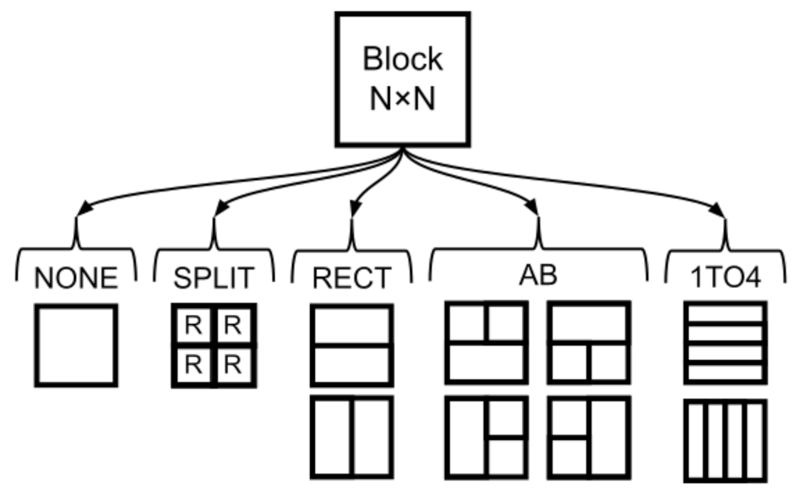
\includegraphics[width=0.5\textwidth]{FIGURES/fig_14.png}
    \caption{Tipos de particionamentos permitidos no formato AV1. Fonte: Elaborada pelo autor.}
    \label{fig:14}
\end{figure}

Dessa forma, é possível calcular o número total de arranjos de árvores existentes para cada superbloco do AV1, que é de 2.555 combinações. Detalhamos o cálculo desse número no Apêndice \ref{apx:B}. Considerando o rol de ferramentas disponíveis para realizar as predições intraquadro ou interquadros no AV1, para todas essas 2.555 combinações, em uma implementação de busca exaustiva, é possível afirmar que a aplicabilidade desse processo de codificação de vídeo seria inviável sem o uso de algum acelerador de hardware dedicado para esse fim. Por essa razão, o software referência do AV1, mesmo em suas versões iniciais, não utiliza algoritmos de busca exaustiva em seus fluxos de execução, optando por condicionais de paradas antecipadas (podas) que permitem a interrupção dos testes. Até a publicação da versão 2.0 do software de referência do AV1 (\textit{libaom}), as podas eram realizadas por técnicas baseadas em análises estatísticas. Desde então, as novas versões do software de referência utilizam modelos de aprendizado de máquina para predizer as podas, conforme descrito em \citet{bib:av1_ml_partitioning}.

Dessa forma, duas análises distintas precisam ser feitas sobre o AV1. A primeira sobre o custo computacional da execução do codificador de referência do AV1 sob diferentes estruturas de particionamento (seção \ref{cap:5.1}) e a segunda sobre a distribuição de ocorrências da subdivisão dos blocos em quatro novos ramos (modo SPLIT) na árvore de particionamentos (seção \ref{cap:5.2}).

\section{Complexidade das Estruturas de Particionamento}
\label{cap:5.1}

Para avaliar o custo computacional do processo de particionamento de blocos do formato AV1, realizou-se uma série de experimentos. Para a realização desses experimentos, foi utilizada a versão do \textit{libaom} disponível no momento inicial da pesquisa apresentada nesta tese (v1.0.0). Note-se que esta versão é diferente da utilizada nas etapas finais da pesquisa apresentada nesta tese, que é mais atualizada (como vimos na seção \ref{cap:4.2}). Apesar da versão 3.5.0 ser 61\% mais rápida que a versão 1.0.0 e apresentar um aumento de 4,07\% de BD-rate, conforme experimentos próprios realizados com cinco vídeos HD1080, as proporções gerais de complexidade observadas neste capítulo tendem a se manter.

O experimento realizado consiste em ativar e desativar ferramentas do \textit{libaom}, em uma estratégia conhecida como \textit{tool-on/off analysis}. Como o objetivo consiste em analisar as estruturas de particionamento, focamos em avaliar os parâmetros do \textit{libaom} que permitem a manipulação da árvore de particionamento. Assim, foi possível definir as 18 variações de parâmetros descritas na Tabela \ref{tab:VIII}. Podem ser observadas diversas variações, como ativar ou desativar os tipos \textit{RECT}, \textit{AB} e \textit{1TO4} (respectivamente, os parâmetros \texttt{enable-rect-partitions}, \texttt{enable-ab-partitions} e \texttt{enable-1to4-partitions}) ou realizar alterações diretas nas profundidades da árvore de particionamentos do AV1, através do tamanho de bloco quadrático máximo (\texttt{max-partition-size}) e mínimo (\texttt{min-partition-size}) permitidos. Neste último caso, existe uma restrição crítica: o valor mínimo do tamanho quadrático deve ser sempre menor que o valor máximo. Na Tabela \ref{tab:VIII}, também é apresentado o total de combinações de árvores que o AV1 poderá dispor para testes (considerando o algoritmo descrito no Apêndice \ref{apx:B}).

\afterpage{
\clearpage

\begin{landscape}
{\footnotesize
\begin{longtblr}[
    caption = {Experimentos de \textit{tool-on/off analysis} das árvores de particionamento do \textit{libaom}.},
    label = {tab:VIII}
]{
    colspec = {c|l|c|r|r|r},
    rowhead = 1,
    hlines,
    row{even} = {gray9}
}
\hline
\textbf{Combinação} & \textbf{Parâmetro} & \textbf{Arranjos Máximos de Árvores} & \textbf{BD-rate (\%)} & \textbf{TS (\%)} & \textbf{Razão}\\

0 & Referência & 2555 & \SetCell[c=1]{c}-~- & \SetCell[c=1]{c}-~- & \SetCell[c=1]{c}-~-\\
1 & -~-enable-rect-partitions=0 & 1365 & 4,81 & 36,22 & 0,133\\
2 & -~-enable-ab-partitions=0 & 2215 & 0,39 & 12,88 & 0,030\\
3 & -~-enable-1to4-partitions=0 & 2387 & 0,33 & 13,20 & 0,025\\
4 & -~-sb-size=64 & 2548 & 0,49 & 15,49 & 0,032\\
5 & -~-min-partition-size=64 -~-max-partition-size=128 & 43 & 92,68 & 65,75 & 1,409\\
6 & -~-min-partition-size=32 -~-max-partition-size=128 & 187 & 30,17 & 39,81 & 0,758\\
7 & -~-min-partition-size=16 -~-max-partition-size=128 & 763 & 8,03 & 24,13 & 0,333\\
8 & -~-min-partition-size=8 -~-max-partition-size=128 & 1531 & 0,45 & 14,15 & 0,032\\
9 & -~-min-partition-size=32 -~-max-partition-size=64 & 180 & 30,65 & 53,57 & 0,572\\
10 & -~-min-partition-size=16 -~-max-partition-size=64 & 756 & 8,57 & 35,49 & 0,241\\
11 & -~-min-partition-size=8 -~-max-partition-size=64 & 1524 & 0,95 & 20,13 & 0,047\\
12 & -~-min-partition-size=4 -~-max-partition-size=64 & 2548 & 0,48 & 17,40 & 0,027\\
13 & -~-min-partition-size=16 -~-max-partition-size=32 & 720 & 14,27 & 49,58 & 0,288\\
14 & -~-min-partition-size=8 -~-max-partition-size=32 & 1488 & 6,49 & 36,39 & 0,178\\
15 & -~-min-partition-size=4 -~-max-partition-size=32 & 2512 & 6,06 & 33,61 & 0,180\\
16 & -~-min-partition-size=8 -~-max-partition-size=16 & 1344 & 28,90 & 60,31 & 0,479\\
17 & -~-min-partition-size=4 -~-max-partition-size=16 & 2368 & 28,35 & 55,80 & 0,508\\
18 & -~-min-partition-size=4 -~-max-partition-size=8 & 1792 & 103,56 & 76,66 & 1,351\\
\hline
\end{longtblr}
}
\end{landscape}
}


Foram realizados, portanto, 19 experimentos, os 18 experimentos descritos na Tabela \ref{tab:VIII}, além da codificação de referência (00) usada como base para as comparações. Todas essas codificações utilizam as mesmas configurações padrões do \textit{libaom} e utilizam quatro vídeos HD1080, conforme descrição detalhada realizada na seção \ref{cap:4.1}. Mesmo sem executar os experimentos, a Tabela \ref{tab:VIII} permite especular que a combinação 05 (testar apenas as profundidades 0 e 1) tende a ser a mais rápida, por possuir poucos arranjos de árvores para realização de testes preditivos (apenas 43). Em termos de redução de tempo de codificação, a combinação 05 deve ser seguida da combinação 09 (testar apenas as profundidades 1 e 2), pois esta possui 180 variações de árvores. No entanto, apesar de esses dois experimentos possuírem poucas possibilidades de árvores disponíveis para avaliação, as etapas de predições possuem custos de processamento diferentes, a depender do tamanho do bloco, o que influencia no tempo total de codificação. Por outro lado, os experimentos 04 e 12 tendem a apresentar resultados iguais, pois ambos possuem o mesmo número de árvores disponíveis para teste, inclusive com configurações praticamente idênticas. Na Tabela \ref{tab:VIII}, também constam os resultados obtidos com a execução dos experimentos, onde são mostrados valores de BD-rate e TS (vide equação 7).

Como mencionado anteriormente, esperava-se que as combinações 05 e 09 apresentassem os maiores valores de TS de todo o conjunto de experimentos. Todavia, isso não é o que se observa na Tabela \ref{tab:VIII}. As combinações com os maiores valores de TS foram as de número 18, 05 e 16, com a combinação 09 aparecendo apenas em quinto lugar. O maior destaque é para a combinação 18, com uma redução de complexidade de 76,66\%, o que se dá pela sua limitação: o codificador só tem à sua disposição blocos pequenos (8$\times$8 ou menores). Em termos gerais, processar os estágios de predição em blocos pequenos tende a ser computacionalmente menos custoso que em blocos maiores, como é possível observar com os dois extremos apresentados na Tabela \ref{tab:VIII}, onde vemos 43 árvores distintas na combinação 05 frente a 1792 da combinação 18. Outra parte da explicação para o valor de TS elevado da combinação 18, assim como na 16 (60,31\%), se deve ao percentual de representação dos diferentes tamanhos de bloco em um quadro, conforme discutido anteriormente no capítulo \ref{cap:2}. Naquele capítulo, a Tabela \ref{tab:I} evidenciou que um bloco 8$\times$8 representa uma área de 0.00309\% de um quadro de vídeo HD1080, enquanto blocos 4$\times$4 representam uma área ainda menor (0.00077\%). Logo, as perdas ocasionadas por predições imprecisas nesses casos é menor, tanto em termos de qualidade subjetiva, quanto em termos de qualidade objetiva da imagem. No entanto, há um agravante no uso exclusivo desses tamanhos de bloco: o elevado custo em taxa de bits para representação desses blocos no \textit{bitstream} codificado, justificando o BD-rate elevadíssimo observado no experimento 18.

Enquanto a combinação 18 emprega apenas blocos pequenos e isso impacta significativamente no BD-rate, a combinação 05, que utiliza exclusivamente blocos grandes, também apresenta problemas similares. Apesar de a quantidade de bits para representar a existência de blocos grandes ser significativamente menor, os resíduos da predição interquadros (especialmente) tendem a ser maiores, aumentando a complexidade das etapas seguintes à predição, como o cálculo de transformadas, quantização e codificação de entropia. Além disso, qualitativamente, a imagem resultante é menos agradável ao usuário, visto que sofre maiores perdas.

Na Tabela \ref{tab:VIII}, há outros resultados que merecem destaque, como as combinações que evitam particionamentos quaternários (combinação 03), ternários (02) e binários (01). Esta última combinação, inclusive, desabilita automaticamente as combinações 02 e 03. Os três experimentos apresentaram uma redução de tempo de 13,20\%, 12,88\% e 36,22\%, respectivamente. Como a combinação 01 também desabilita os particionamentos ternários e quaternários, é possível estimar que o particionamento binário possui um impacto aproximado de 10\% do tempo total de codificação do \textit{libaom} (ou seja, a subtração entre 36,22\% e os valores de 12,88\% e 13,20\%). Observa-se na Tabela \ref{tab:VIII} um baixo impacto na eficiência de codificação ao se desabilitar os particionamentos ternários (combinação 02) e quaternários (combinação 03) em vídeos HD1080, inferior a 0,4\% em BD-rate. No entanto, apesar dos particionamentos binários exigirem um tempo de codificação pouco abaixo dos particionamentos ternários e quaternários, o experimento com a combinação 01 indica que a ausência de predições retangulares impacta a codificação com um acréscimo de 4,81\% em BD-rate. Em outras palavras, é importante para a boa eficiência do codificador a disponibilidade dos modos de particionamento retangulares.

Outro ponto anteriormente levantado foi a semelhança entre os experimentos 04 e 12, que levam à mesma configuração no codificador. Apesar de ambos tecnicamente disporem do mesmo arranjo de árvores para codificação, essa igualdade não se replica nos resultados de BD-rate, respectivamente de 0,49\% e 0,48\%, e nem de TS, respectivamente de 15,49\% e 17,40\%. O principal fator que leva a essa diferença nos resultados está no fluxo de execução do próprio \textit{libaom}, que será apresentado na seção \ref{cap:7.4}. Enquanto no experimento 04 o \textit{libaom} parte de um superbloco de 64$\times$64 amostras, iniciando suas variáveis de controle a partir desse tamanho de bloco, a codificação com limitações na árvore (experimento 12) não impede que as variáveis do superbloco sejam iniciadas no bloco quadrático de tamanho 128$\times$128. Consequentemente, o \textit{libaom} dispõe de mais informações para melhor tomada de decisão no segundo caso, o que explica os melhores resultados do experimento 12 em relação ao experimento 04. 

\section{Distribuição de Profundidades e do Modo \textit{SPLIT}}
\label{cap:5.2}

Outro experimento relevante para o desenvolvimento das soluções apresentadas nos capítulos seguintes desta tese é a avaliação da distribuição de profundidades e do uso do modo \textit{SPLIT} na codificação de vídeo segundo o formato AV1. Conhecer quais profundidades tendem a ter maior relevância para a codificação auxilia-nos a considerá-las prioritárias nas tomadas de decisão, principalmente no que se refere ao processo de busca preditiva, seja intraquadro ou interquadros. Também é importante saber a distribuição da utilização do modo \textit{SPLIT} ao longo das profundidades da árvore de particionamento do AV1, pois ela evidencia quais profundidades tendem a ser mais particionadas. Dessa forma, com esses dois dados extras, torna-se possível identificar quais profundidades são mais ou menos interessantes de serem consideradas durante o desenvolvimento de uma solução para codificação ou transcodificação rápida.

Diferentemente do experimento apresentado na seção anterior, a avaliação relatada nesta seção leva em consideração várias decisões tomadas em fases posteriores da tese. Portanto, os resultados apresentados aqui foram obtidos com uma versão atualizada do software de referência do AV1 e consideram 14 sequências de vídeo HD1080 (conforme detalhado na seção \ref{cap:4.1}).

A Figura \ref{fig:16} representa a distribuição das ocorrências de cada uma das profundidades permitidas no formato AV1, considerando os quatro níveis de quantização (vide seção \ref{cap:4.2}) utilizados nos experimentos relatados ao longo desta tese. A Figura \ref{fig:16} foi gerada através de uma comparação da média das áreas de ocorrência de cada uma das profundidades em relação à área total do quadro codificado. Desta forma, é possível observar uma maior utilização da profundidade 1 (bloco quadrático de tamanho 64$\times$64 pixels), exceto quando o CQ é igual a 20, onde há uma opção pela profundidade 2. Em outras palavras, essa observação nos dá indícios de que o codificador AV1 tende a optar pela utilização dos blocos de altura ou largura igual a 64, em algum dos nove tipos de particionamentos disponíveis. Logo, considerando os experimentos realizados na seção anterior, compreende-se a causa do elevado impacto negativo das combinações 13 e 18 ao omitir a disponibilidade dos blocos 64$\times$64. Os experimentos mostram que não permitir o uso dessa profundidade implica, invariavelmente, na distribuição dos blocos em profundidades menores, o que causa um aumento na taxa de bits necessária para representar o vídeo codificado.

\begin{figure}
    \centering
    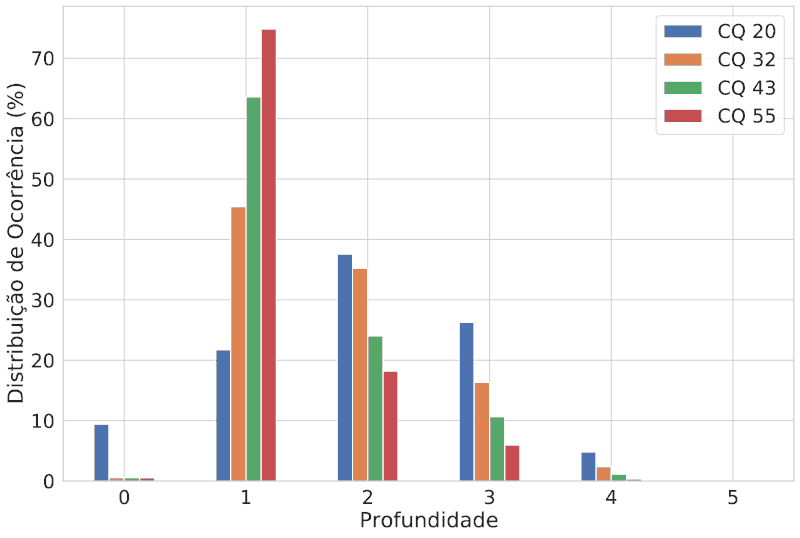
\includegraphics[width=0.75\textwidth]{FIGURES/fig_16.png}
    \caption{Média de distribuição das profundidades da árvore de particionamento do AV1. Fonte: Elaborada pelo autor.}
    \label{fig:16}
\end{figure}

Outra constatação a partir da Figura \ref{fig:16} é a relativa ausência de blocos 4$\times$4, que representam uma área média inferior a 0,3\% dos vídeos HD1080 utilizados nos experimentos. O mesmo pode ser observado com a profundidade 0, que ocupa uma área média inferior a 1\% em quase todos os experimentos realizados com diferentes níveis de quantização, exceto no caso da quantização configurada com CQ 20, onde a área de emprego da profundidade 0 é de 9\%. Essa observação contraria a expectativa de que vídeos codificados com menores parâmetros de quantização tendem a apresentar mais particionamentos; os resultados mostram que neste caso foram utilizados blocos maiores na codificação.

Em complemento à análise de distribuição de profundidades, é importante avaliar também o índice de utilização do modo de particionamento \textit{SPLIT} para cada profundidade da árvore. Essa informação é particularmente útil para definir quais profundidades são mais utilizadas e, consequentemente, quais são os particionamentos que, caso forçados ou evitados, têm potencial de causar maior impacto na eficiência de codificação do software do AV1. Utilizando os mesmos vídeos do experimento apresentado na Figura \ref{fig:16}, a Figura \ref{fig:17} mostra a taxa de uso do modo \textit{SPLIT} para cada profundidade e para cada nível de quantização considerado nos experimentos apresentados nesta tese. Na Figura \ref{fig:17}, os dados estão distribuídos de acordo com duas escolhas: o codificador decidiu pelo bloco naquele nível de profundidade (não-\textit{SPLIT}, em laranja) ou decidiu por subparticionar o bloco (\textit{SPLIT}, em azul). Em cada profundidade considerada (eixo x) o somatório de casos \textit{SPLIT} e não-\textit{SPLIT} é igual ao total de casos \textit{SPLIT} da profundidade anterior. No topo de cada coluna, encontra-se destacado o valor proporcional do modo \textit{SPLIT} (em azul) para aquela profundidade. Desta forma, torna-se possível identificar a probabilidade de ocorrência de particionamentos em cada profundidade e, ao mesmo tempo, identificar quais profundidades são utilizadas, complementando a Figura \ref{fig:16}. Por exemplo, na profundidade 2 (blocos 32$\times$32), considerando uma codificação com CQ 20, o codificador \textit{libaom} opta por subparticionar o bloco em blocos menores em 45,46\% das vezes. Quando processa blocos em profundidade 4, considerando o mesmo CQ 20, em apenas 4,11\% das vezes o codificador opta por subparticionar em blocos menores na profundidade 5.

\begin{figure}
    \centering
    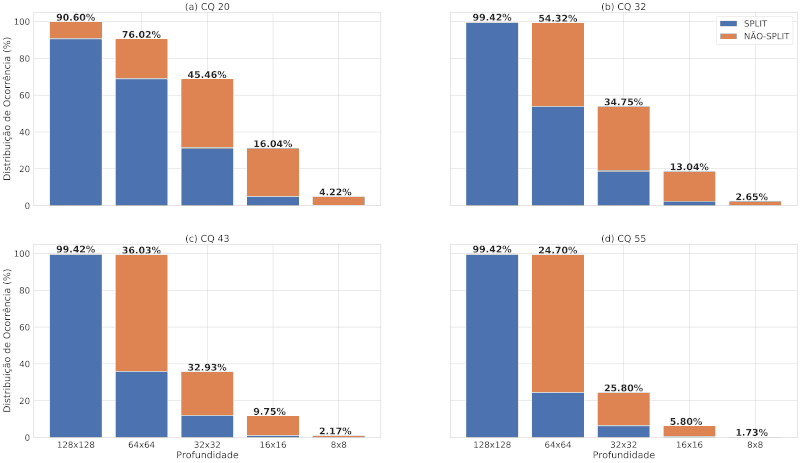
\includegraphics[width=\textwidth]{FIGURES/fig_17.png}
    \caption{Probabilidade do subparticionamento em modo \textit{SPLIT} para cada nível da árvore de particionamento do AV1, em CQs (a) 20, (b) 32, (c) 43 e (d) 55. Fonte: Elaborada pelo autor.}
    \label{fig:17}
\end{figure}

Evidenciamos neste capítulo que a escolha de particionamentos e de tamanhos de blocos influencia consideravelmente o custo computacional do software de referência do AV1 e também a sua eficiência de codificação. Portanto, uma das tarefas essenciais de um codificador ou transcodificador rápido, quando baseado em escolhas de particionamentos, é identificar a melhor combinação de blocos sem a necessidade de realizar um grande número de testes. Nesse sentido, o capítulo \ref{cap:6} contempla as primeiras soluções desenvolvidas no escopo desta tese, que envolvem transcodificadores rápidos por heurísticas baseados em análises estatísticas. No capítulo \ref{cap:7}, apresentamos a proposta de transcodificador rápido baseado no reaproveitamento de estruturas de particionamento com uso de modelos preditivos gerados por algoritmos de aprendizado de máquina, aplicados a diversos transcodificadores.
